\documentclass{handout_utfpr}

\usepackage{xspace}
\usepackage{pbox}
\usepackage[brazil]{babel}
\usepackage{xcolor}
\usepackage[alf]{abntex2cite}
\usepackage{pdfpages}
\usepackage{url}
\usepackage{geometry}
\usepackage{dashrule}
\usepackage{listings}
\definecolor{dark-gray}{gray}{0.20}
\definecolor{light-gray}{gray}{0.85}

\newcommand{\com}[1]{
\colorbox{light-gray}{\texttt{\pbox{\textwidth}{\$ #1}}}
}

\newcommand{\cominline}[1]{
\colorbox{light-gray}{\texttt{\pbox{\textwidth}{#1}}}
}

\newcommand{\pdf}{\textsf{.pdf}}
\newcommand{\dvi}{\textsf{.dvi}}
\newcommand{\tex}{\textsf{.tex}}

\subjnum{CC31C}
\subject{Introdução à Ciência da Computação}
\subjelab{Introdução ao \LaTeX}

\handoutdate{\today}

\begin{document}
\maketitle

\section{Introdução}

Este material é apresentado como parte de uma série de minicursos que serão ministrados sobre tópicos variados com o intuito de \textit{nivelar} o conhecimento dos alunos com relação a conceitos básicos que não estão inclusos nas ementas das disciplinas regulares do curso, bem como colocá-los em contato com ferramentas úteis e boas práticas da Computação.

Os conteúdos são dispostos aqui apenas como um apanhado geral com o objetivo de prover um embasamento mínimo e recomenda-se que outras fontes de pesquisa sejam utilizadas para o aprofundamento nestes assuntos.



\subsection{A escrita científica}
A necessidade da escrita científica é constante. Na universidade, ela é tida como o principal meio de troca de informações %entre as diferentes partes envolvidas 
no processo de difusão do conhecimento. Autores a utilizam em seus livros, pesquisadores divulgam suas descobertas através da publicação em revistas científicas, professores verificam o desempenho de seus alunos em avaliações escritas e os próprios acadêmicos a utilizam durante seus estudos. Na indústria, a escrita é valorizada na forma de relatórios técnicos, documentação de software e especificação de produtos.

Devido à sua importância, é natural que existam certas diretivas para se produzir um texto de forma correta e aqueles que não estão habituados a estas regras muitas vezes encontram dificuldades. Um problema frequente é o da apresentação visual dos documentos. No ambiente acadêmico, o interesse está no conteúdo de um trabalho e não em sua estética. Os artigos devem ser formatados seguindo uma norma padrão, geralmente definida pela instituição ou evento/revista no qual o trabalho está sendo divulgado. 

\subsection{Normas para escrita de trabalhos científicos}
A normas são definidas não de maneira aleatória, mas levando em consideração vários fatores como legibilidade do texto, tamanho do documento, local de publicação, presença de fórmulas matemáticas ou imagens, etc. Alguns dos detalhes presentes nas normas para escrita de artigos e trabalhos acadêmicos são: requisitos com relação à fontes, à disposição de parágrafos e seções, exibição de fórmulas e figuras, formatação de sumário e bibliografia.

Como estes detalhes são difíceis de serem capturados em palavras e regras, mostra-se abaixo um mesmo documento formatado de maneira a atender as regras de formatação do {\slshape Institute of Electrical and Electronics Engineers} (\textbf{IEEE}, acima) e da Sociedade Brasileira de Computação (\textbf{SBC}, abaixo).

Observe na página seguinte as diferenças com relação aos elementos de formatação do texto:
\begin{itemize}
\item Margens.
\item Estilos e tamanhos de fonte.
\item Centralização.
\item Forma de apresentar o nome dos autores.
\item Numeração das seções.
\item Tabulação dos parágrafos.
\end{itemize}

% Como exemplo do formato utilizado no padrão de conferências do IEEE, a página \pageref{IEEE} mostra o estilo de formatação necessário para submissão. Este formato é muito requisitado nos congressos internacionais e até mesmo para alguns eventos da SBC.

% No entanto, alguns congressos da SBC utilizam também formato próprio. Esse formato pode ser analisado na página \pageref{SBC}

Além disso, outro detalhe importante é a seção de referências. Cada congresso dispõe de maneiras diferentes para apresentação e citação das mesmas. Após a comparação entre a formatação dos textos, mostra-se, na página \pageref{referencias} as diferenças entre as referências das normas.

Repare como a citação do IEEE, na parte superior, ainda utiliza o formato de duas colunas, possui citação numérica, cita mais do que um autor e mostra maiores informações sobre a publicação em si. A norma da SBC, no meio, se parece mais com o padrão da UTFPR por ambas terem base na ABNT. As citações são por nome do autor e ano da publicação, e com menos informações sobre a obra. Por fim, as normas da UTFPR ressaltam o congresso publicado em negrito, autor todo em maiúsculo e mais metadados.

{\clearpage
\label{cabecalhos}
\newgeometry{left=0cm,bottom=0cm,top=0cm,right=0cm}

\noindent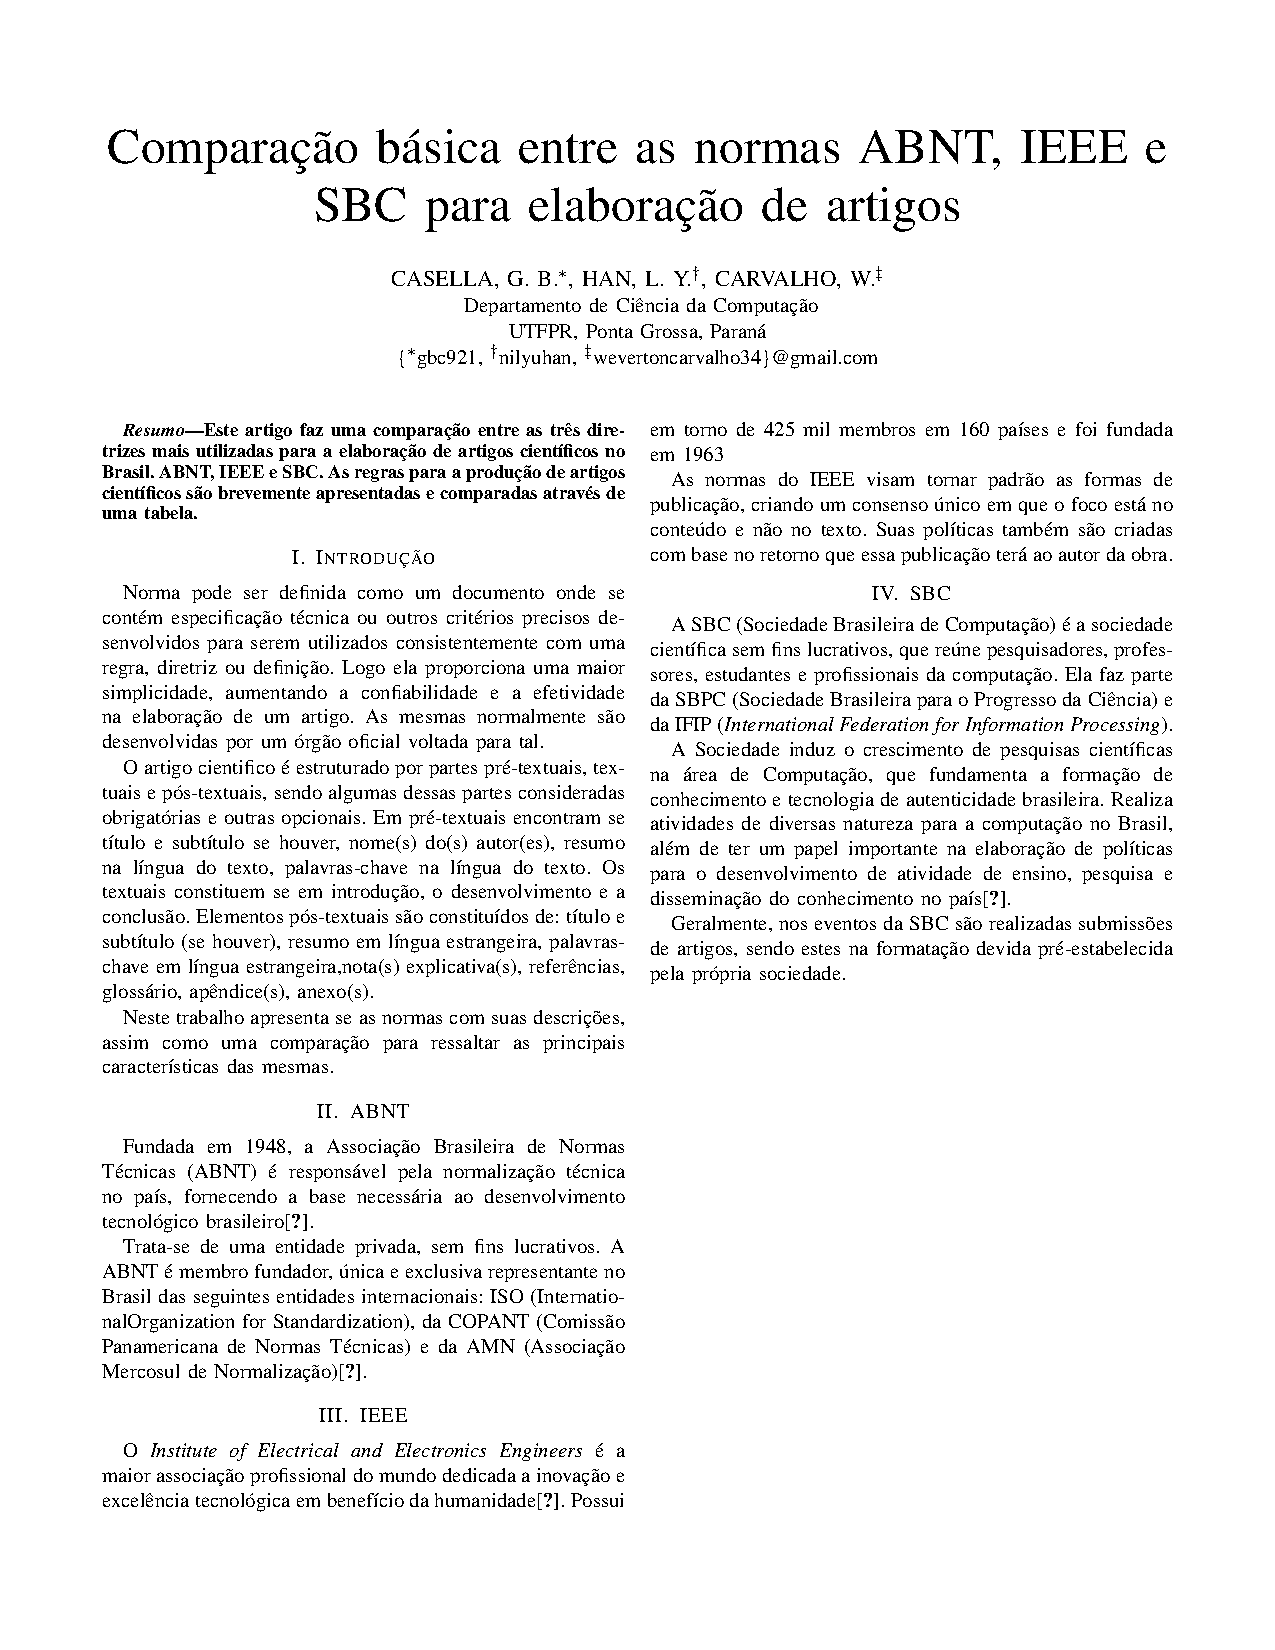
\includegraphics[trim=0 15cm 0 0,clip]{conteudo/intro_modelo_conferencias/intro_writing_ieee}

\hrule
%\noindent\hdashrule[0.5ex]{\textwidth}{2pt}{10pt}

\noindent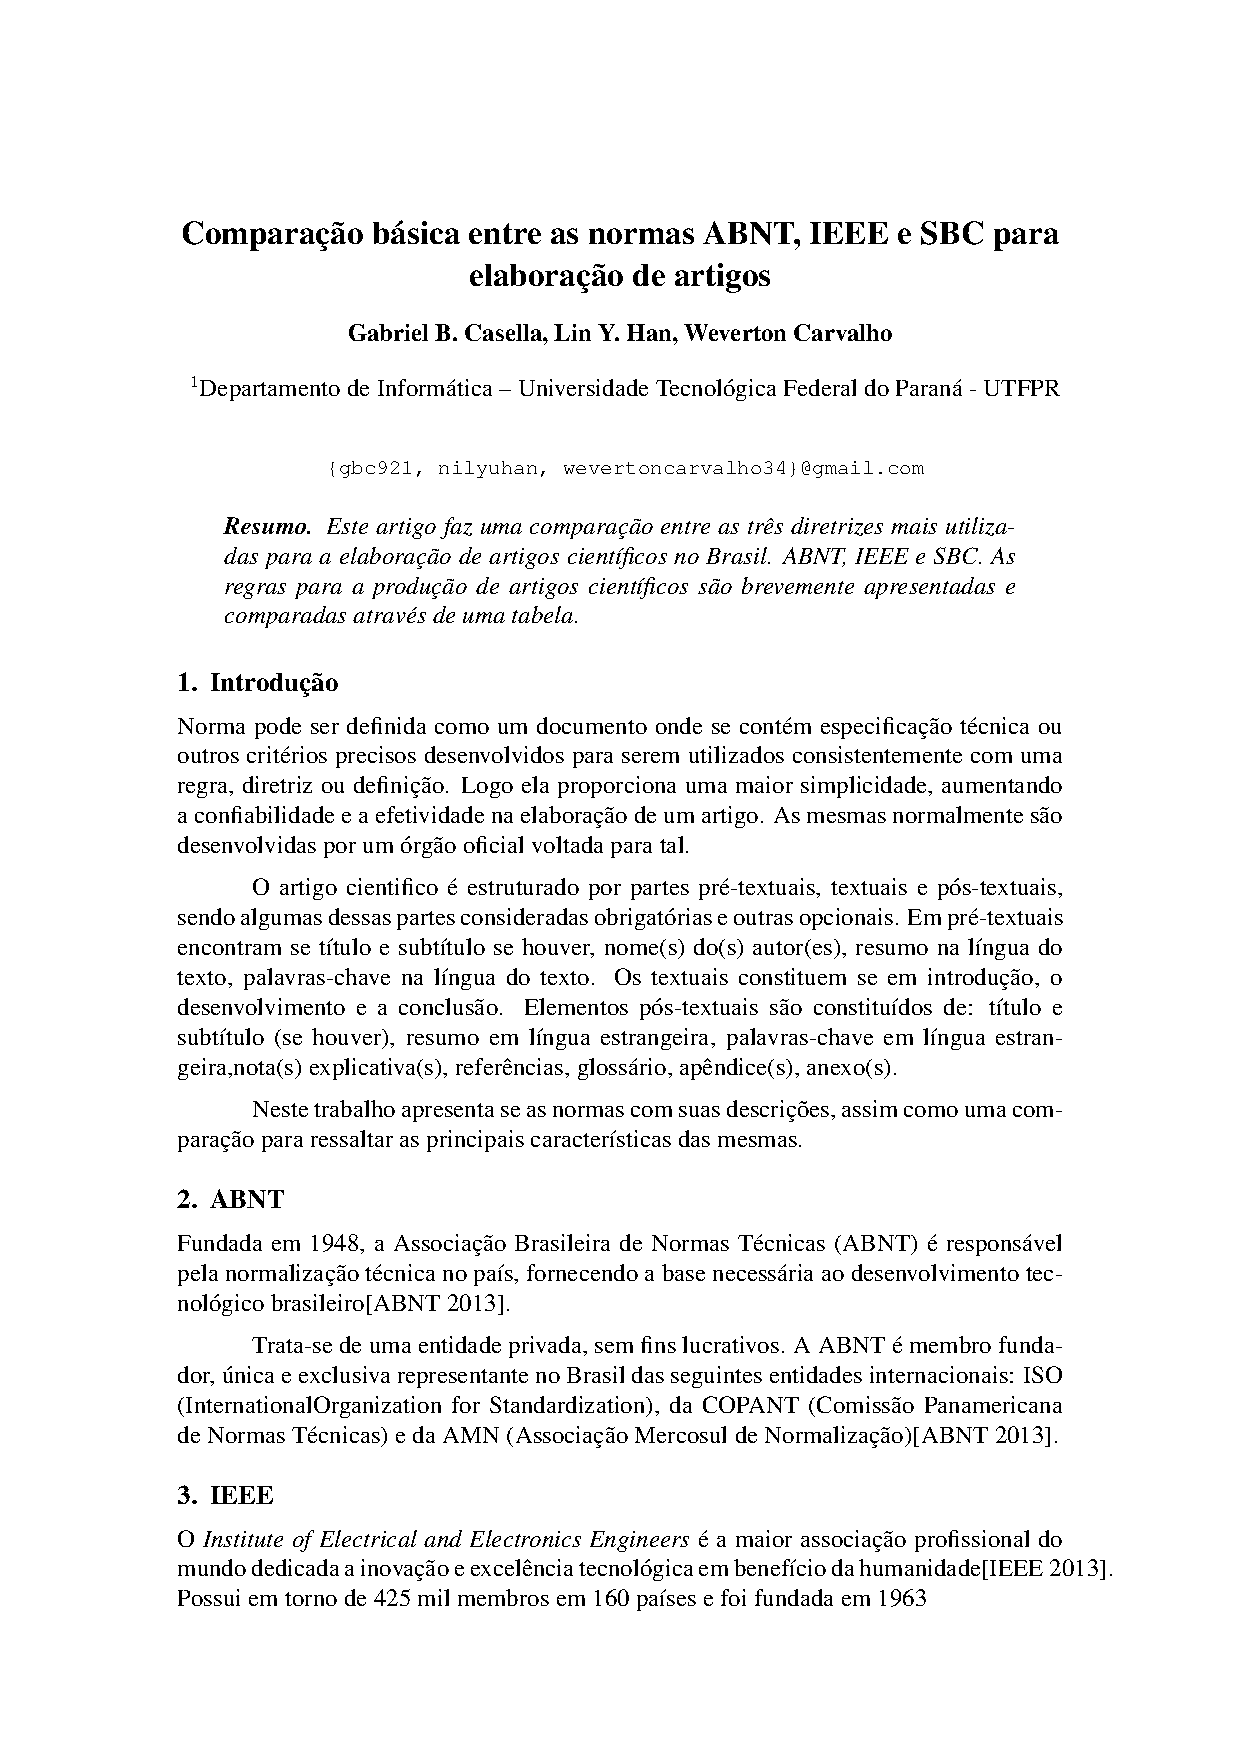
\includegraphics[trim=0 15cm 0 0,clip]{conteudo/intro_modelo_conferencias/intro_writing_sbc}

\clearpage}
\restoregeometry

 %Estes são apenas alguns dos detalhes que são exigidos e fica claro que a correta formatação de um documento é um processo que acaba ocupando uma grande parte do tempo dedicado à escrita do mesmo e 

{\clearpage
\label{referencias}
\newgeometry{left=0cm,bottom=0cm,top=0cm,right=0cm}

\noindent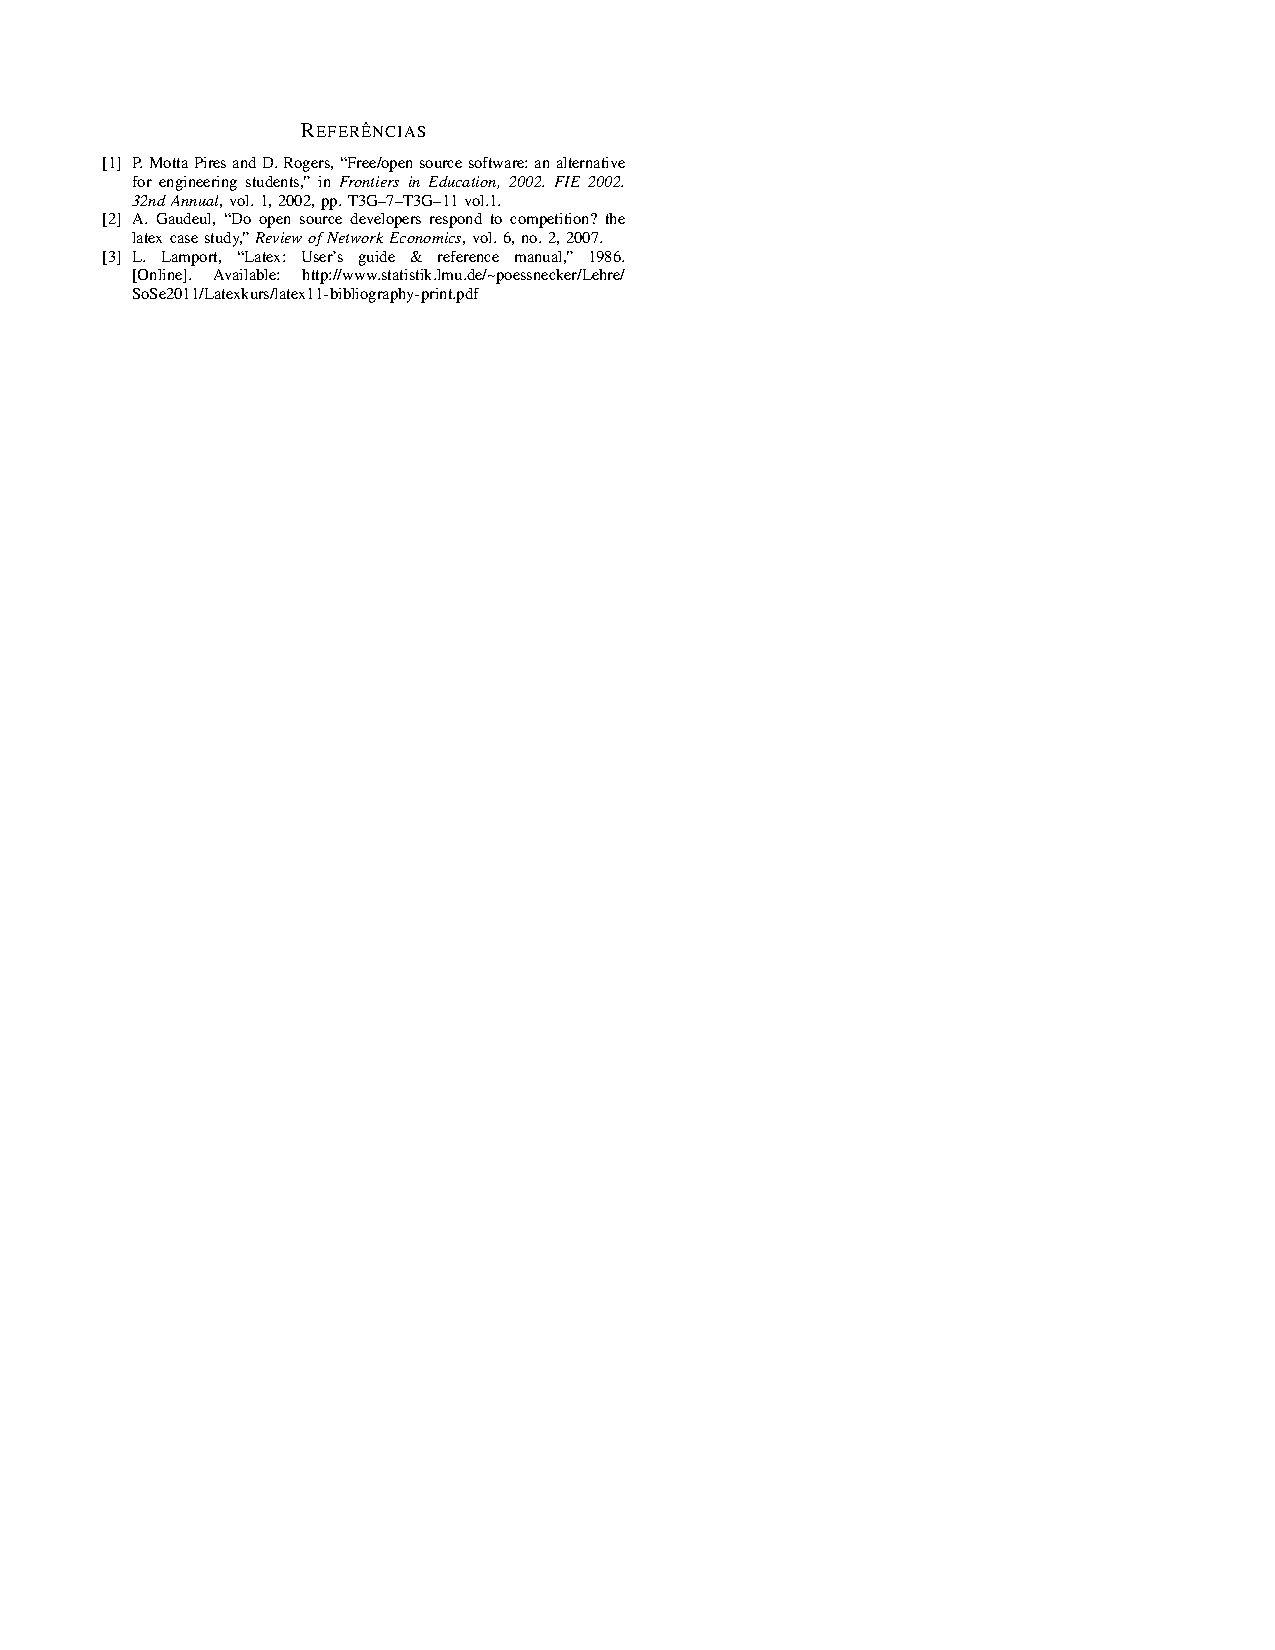
\includegraphics[trim=0 19cm 0 0,clip]{conteudo/intro_modelo_conferencias/references/ieee-refs}

\hrule

\noindent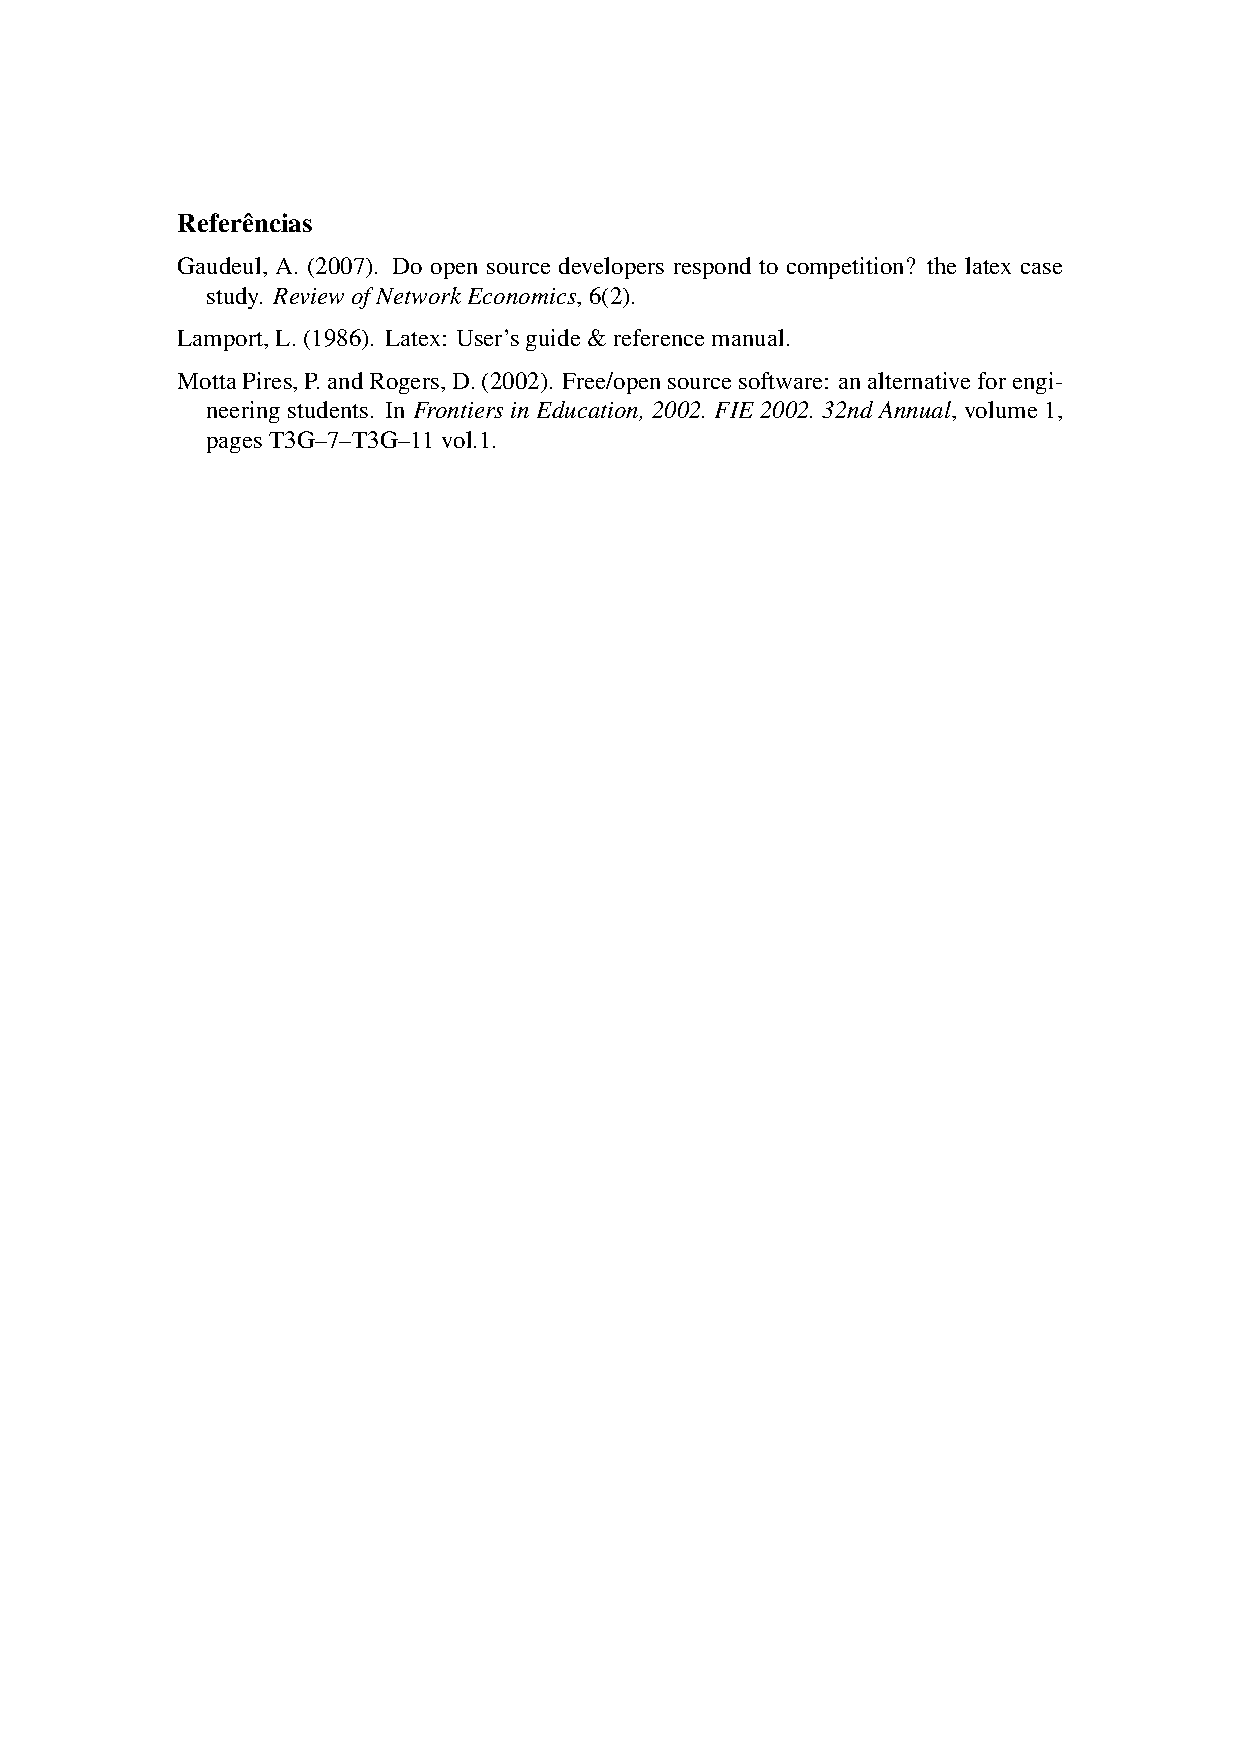
\includegraphics[trim=0 19cm 0 2cm,clip]{conteudo/intro_modelo_conferencias/references/sbc-refs}

\hrule
\noindent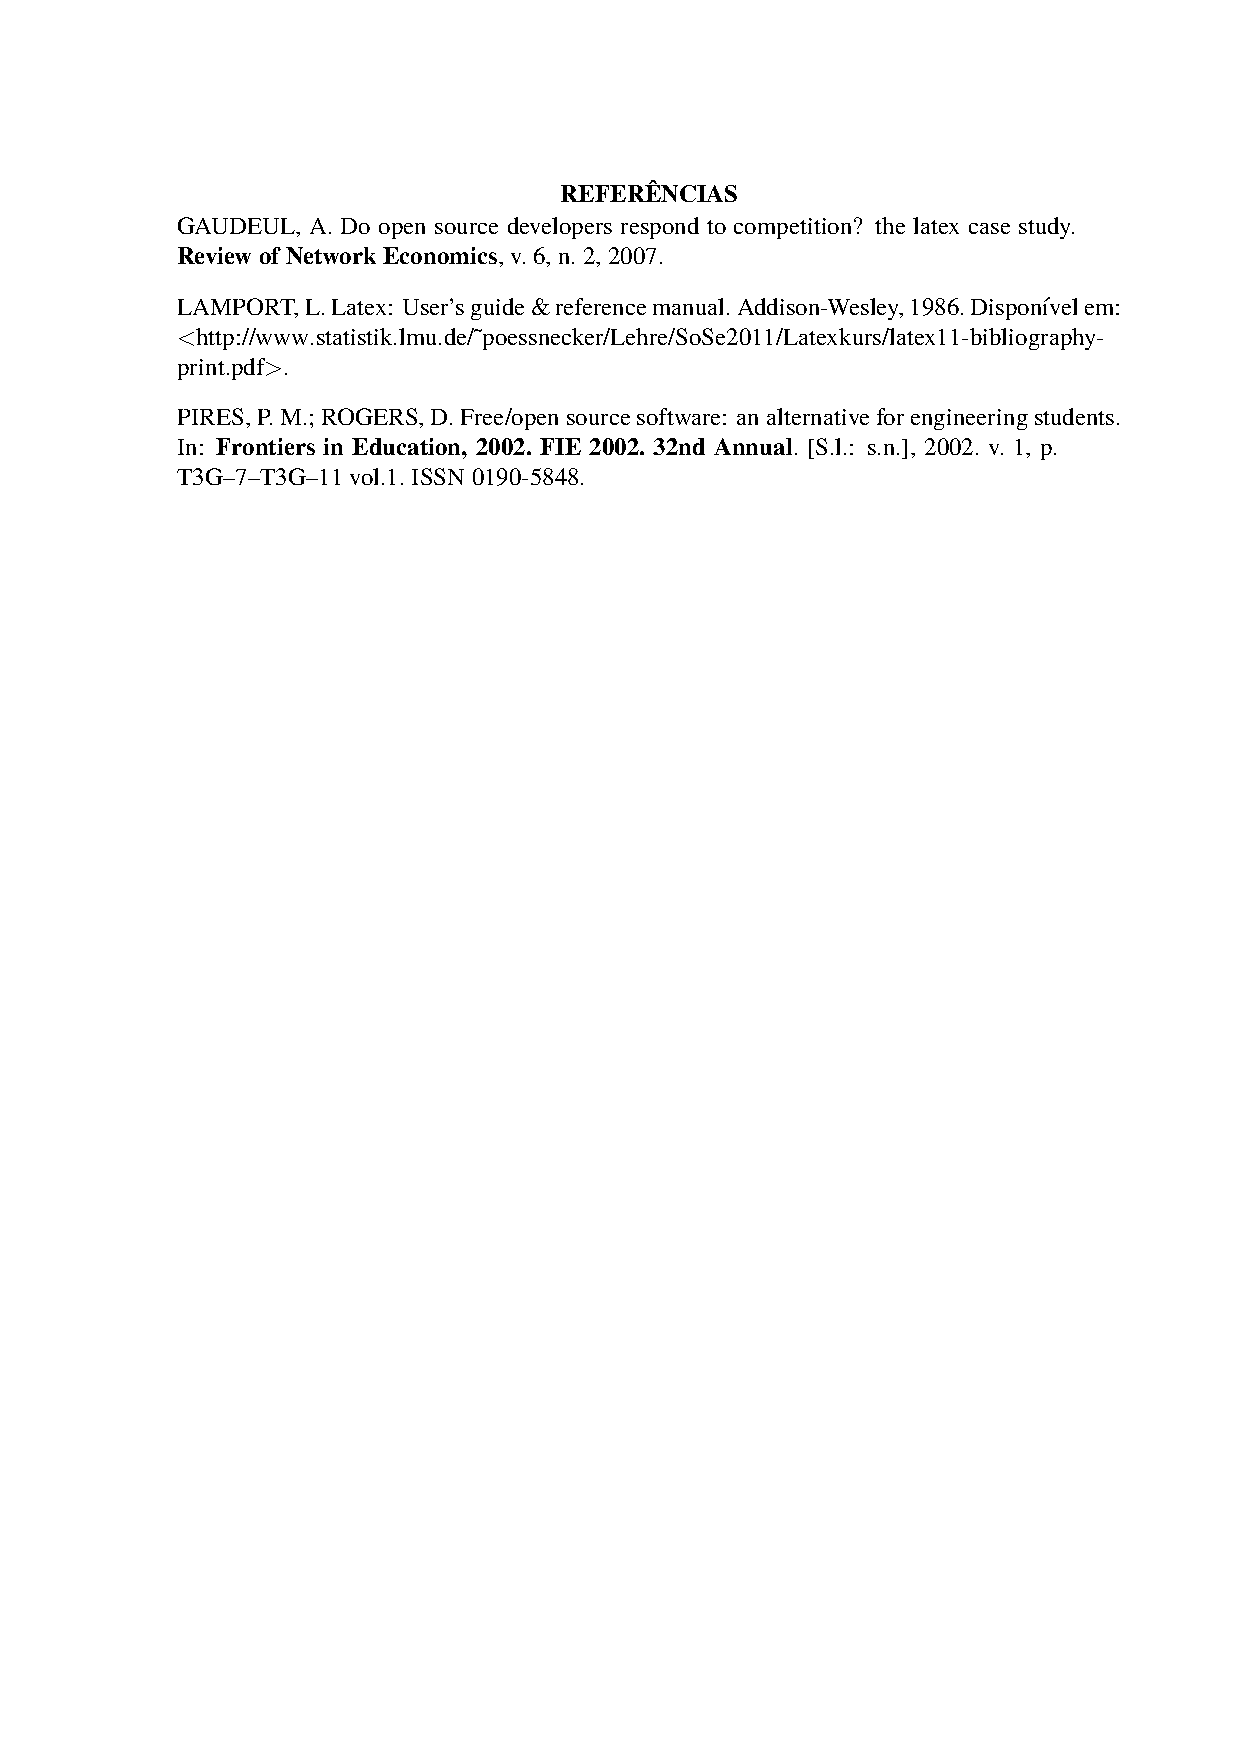
\includegraphics[trim=0 20cm 0 0cm,clip]{conteudo/intro_modelo_conferencias/references/utf-refs}

\clearpage}
\restoregeometry

Tendo em vista todos estes detalhes a serem levados em consideração bem como o fato de que os textos muitas vezes são escritos de maneira apressada devido a prazos curtos, como no caso de artigos ou relatórios de iniciação científica, fica claro que a utilização de ferramentas que automatizem e facilitem este processo de formatação serão sempre bem vindas. Uma destas ferramentas é o \LaTeX.

%Estes são apenas alguns dos detalhes que são exigidos e fica claro que a correta formatação de um documento é um processo que acaba ocupando uma grande parte do tempo dedicado à escrita do mesmo e a utilização de ferramentas que automatizem e facilitem este processo são sempre bem vindas. Uma destas ferramentas é o \LaTeX.


 % Introdução à escrita científica

\section{\LaTeX}
O \LaTeX é um sistema para a editoração de documentos de alta qualidade tipográfica. Utiliza-se do \TeX, um programa que foi criado pelo matemático Donald Knuth que, ao revisar o segundo volume da sua série de livros {\slshape The Art of Computer Programming} verificou que a sua qualidade era muito baixa e já que a produção de um texto em formato digital era basicamente uma combinação de zeros e uns (com tinta e sem tinta), decidiu criar um sistema próprio.

Knuth inicialmente previu que a sua tarefa, que consistia em aprender quais eram as formas tradicionais de se exibir fórmulas matemáticas, a maneira correta de se imprimir letras em um papel, como criar suas próprias fontes e por fim integrar tudo isso em um programa de computador, levaria aproximadamente 6 meses. Donald levou quase 10 anos e o produto final de seu trabalho foi o sistema \TeX \ e o programa de criação de fontes \textit{Metafont}.

\LaTeX é basedo na filosofia de que autores devem se focar no conteúdo sem precisar se preocupar com a apresentação visual do que estão escrevendo. Desta forma, ao escrever um documento usando \LaTeX, o autor precisa apenas especificar a estrutura lógica de seu texto, na forma de conceitos básicos como capítulos, seções, tabelas, figuras, etc. A apresentação fica a cargo do sistema.

%LaTeX can be arbitrarily extended by using the underlying macro language to develop custom formats. Such macros are often collected into packages, which are available to address special formatting issues such as complicated mathematical content or graphics. Indeed, in the example below, the align environment is provided by the amsmath package.

\subsection{Funcionamento}

O funcionamento do \LaTeX é o seguinte: a partir de um arquivo de texto com extensão \tex\ contendo comandos e o texto que se quer exibir, o programa \textsf{latex} produz um arquivo independente de plataforma \dvi. Este arquivo então é convertido para diversos formatos dependendo de sua utilização desejada. No caso de uso mais comum, o arquivo \dvi\ é convertido para \pdf. Para se evitar este processo de conversão, normalmente utiliza-se o comando \textsf{pdflatex} que gera o \pdf\ diretamente a partir do \tex.

Um exemplo de sintaxe dos comandos \TeX\ é visto a seguir:
\lstinputlisting{conteudo/exemplo.tex}

Este trecho de código produz um \pdf\ com esta aparência:

\noindent\makebox[\textwidth]{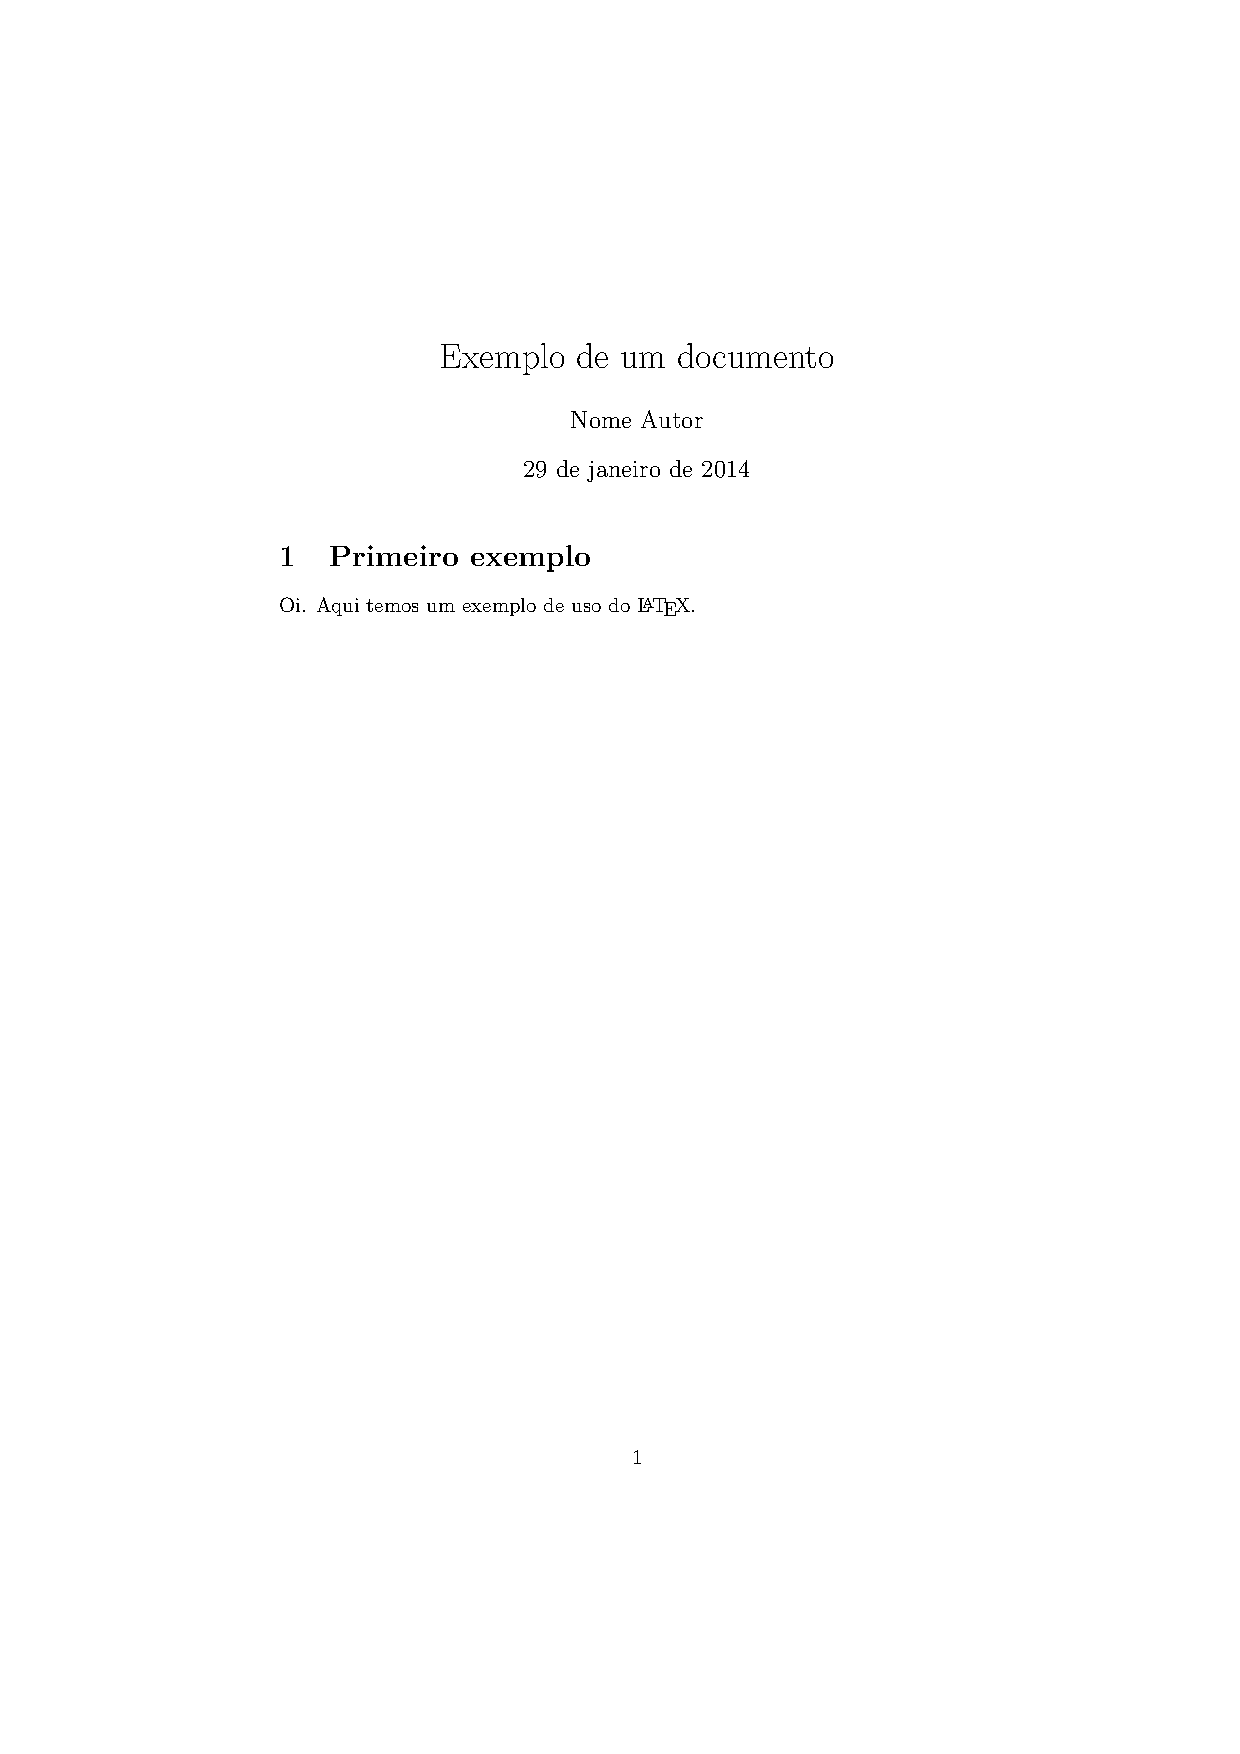
\includegraphics[trim= 0 18cm 0 5cm,clip]{conteudo/exemplo}}

Observe como, no código apresentado, não há nenhuma informação sobre que tipo de fonte utilizar, tamanho da letra, espaçamento entre linhas, posicionamento do título, etc. Estes detalhes são tratados pelo \LaTeX\ e o usuário não precisa se preocupar com eles. % TeX ao resgate!

\subsection{Instalação}
%\subsubsection{Versões}
De acordo com o funcionamento descrito, o \LaTeX nada mais é do que um compilador, convertendo comandos e texto no formato final de apresentação escolhido. Sendo assim, existem compiladores diferentes para cada sistema operacional e várias implementações diferentes baseadas originalmente no \LaTeX/\TeX. Para citar dois exemplos, temos Xe\TeX\cite{xetex}, que possui melhor suporte a fontes e tipografias e 
Lua\TeX que inclui a linguagem de script Lua e é baseada no \textsf{pdflatex}.

Utilizaremos basicamente nesse minicurso o \textsf{pdflatex} que caracteriza-se basicamente por ser uma extensão do \TeX. Para instalação no Windows normalmente utiliza-se a implementação MiK\TeX\cite{miktex} que pode ser baixada aqui \url{http://miktex.org/download}. Este pacote pode automaticamente baixar as os plugins (extensões do \LaTeX) que forem necessárias para funcionamento.

Para ambientes Linux a maioria das distribuições inclui um pacote a ser instalado pelo próprio gerenciador de pacotes da distro. Normalmente é utilizado o \TeX Live que agrega os compiladores, plugins, macros e fontes.

Nos sistemas Debian e derivados (Ubuntu) o \LaTeX pode ser instalado pelos pacotes \textsf{texlive}, \textsf{texlive-base} ou pelo meta-pacote \textsf{texlive-full}. Para o Ubuntu, ainda existe um \textit{script} de instalação\cite{intall-tl-ubuntu} para obter a última versão do \TeX Live (atualmente 2013). A URL de acesso com instruções de instalação pode ser acessada em \url{https://github.com/scottkosty/install-tl-ubuntu}.

Finalmente, para edição dos textos utiliza-se um editor próprio para textos \LaTeX de forma a facilitar o uso dos comandos e macros disponíveis. Dentre os vários disponíveis\cite{wiki:texEditors} utilizaremos aqui o TeXStudio\cite{texstudio} que pode ser baixado em \url{http://texstudio.sourceforge.net/}. O TeXStudio possui várias algumas funções que facilitam na edição de textos, como compilação integrada, visualizador rápido do pdf, \textit{auto-complete} de comandos, dicionário, localização de erros no \textsf{.tex}, entre outros. % Básicos da instalação

\section{WYSIWYG}

A maioria dos softwares responsáveis por processamento de palavras utilizam uma interface que permite que o usuário veja algo muito similar ao resultado final enquanto o documento está sendo criado. Essa interface pode ser chamada de WYSIWYG (``What You See Is What You Get'', ou em uma tradução literal, ``O que você vê é o que você obtém''). Um exemplo de programa que se encaixa nesta classificação é o \textbf{MS Word}.

Em editores WYSIWYG, pedaços de códigos são inseridos no documento para indicar onde a fonte deve mudar de tamanho, onde usar itálico, ou negrito, etc. Esses pedaços de código não são vistos pelo usuário em momento algum, portanto só é possível editar esse arquivo utilizando o próprio software que o criou. Com o \LaTeX, o documento consiste de apenas um arquivo de texto, que pode ser modificado com qualquer editor. É possível dizer, então, que WYSIWYW (``What You See Is What You Want'', ou ``O que você vê é o que você quer'').

\subsection{\LaTeX\ vs WYSIWYG}%Por que o \LaTeX é melhor que softwares WYSIWYG?} 
Embora existam diversas situações onde a utilização de um programa é preferida à de outro por inúmeras razões, existem alguns motivos que podem servir como motivação na escolha do \LaTeX\ como sua ferramenta para criação de textos.

\begin{itemize}
\item Velocidade.

Qualquer ação que requer um mouse ou cliques para acesso de menus será mais lento do que digitar algumas teclas do teclado. Isso significa que digitar caracteres especiais, como uma letra grega, ou principalmente funções serão muito mais rápidos no \LaTeX.

Na edição de arquivos muito grandes, e com muitas figuras e equações, o MS Word, por exemplo, se torna muito mais lerdo, já que ações como mover a barra de rolagem de arquivos pesados requerem muito do processador e da memória. Editar um simples arquivo de texto já não causa tantos problemas para a máquina e a modificação pode ser feita rapidamente.

\item Segurança.

Os arquivos dos editores comuns são armazenados em uma forma binária. Se este arquivo for corrompido por qualquer motivo, o usuário pode perder muitas horas de trabalho. Com arquivos de texto, como no \LaTeX, se um editor falhar, basta abrir o arquivo em outro.

\item Separação de conteúdo e formatação.

A separação em seções e subseções de texto no \LaTeX\ torna muito mais fácil para o escritor se concentrar no texto e na sua ordem de apresentação do que em detalhes superficiais como tamanhos de fonte e estilos.

\item Integração com Sistema de Controle de Versões.

  O \LaTeX\ propicia o uso de sistemas de controles de versão, já que seu formato em texto puro pode ser gerenciado de forma simples por estes sistemas. Desta forma a cooperação entre múltiplos usuários durante a escrita de um texto se torna mais fácil.

  %que precisam integrar o seu projeto em um só, o \LaTeX\ se torna essencial simplesmente pelo seu texto simples, dessa forma também armazenando pouco espaço no servidor. A comparação de dois arquivos usando o ``diff'' também pode ser realizada muito mais facilmente do que no Word, por exemplo.

\item Controle

Alguns editores WYSIWYG possuem configurações prévias que almejam facilitar a digitação de um texto e nestes casos os editores agem sem permissão do usuário, por exemplo: auto-capitalizando as primeiras palavras de uma frase ou selecionando automaticamente sentenças inteiras. Muitas vezes essas edições são indesejadas como no caso dos sinais de subtração, hífen e travessão. Os símbolos -, -- e --- representam três coisas diferentes e quando detalhes deste tipo fazem diferença no contexto da frase, como é frequente em textos científicos, o editor de texto acaba se tornando um problema.

\item Flexibilidade

Por possuir um formato de texto simples, o \LaTeX\ permite a utilização do vasto ferramental que está disponível para a manipulação de arquivos de texto, como por exemplo, substituição usando expressões regulares. Além disso, este formato permite que um arquivo .tex seja transportado de forma flexível e compilado em qualquer ambiente que possua o \LaTeX\ instalado. Modificações no texto também são bastante simples já que o sistema faz a numeração de seções automaticamente, bem como indexação de termos e geração de sumário.

\end{itemize}

Estas são apenas algumas das vantagens deste sistema sobre os editores de texto convencionais e muitos outros detalhes existem, principalmente quanto mais técnico é o conteúdo da escrita. Porém, não seria correto afirmar que o \LaTeX\ é melhor em todos os sentidos que editores WYSIWYG, já que em várias situações, a simplicidade de operação dos editores convencionais faz com que eles sejam melhores em certas tarefas, como quando se deseja fazer um protótipo de design. As interações estéticas são muito mais fáceis de serem percebidas no editor WYSIWYG, porém a manutenção do conteúdo de acordo com o design se torna mais difícil. A escolha, portanto de uma ferramenta certa para a ocasião e para a aplicação que se deseja é importante.

 % Problemas comuns dos editores WYSIWYG

%\input{conteudo/pratica} % Parte prática

\section{Conclusão e dicas finais}
Brevemente apresentou-se a parte lógica de como o \LaTeX\space funciona, qual seu foco principal, onde e porque utilizar, instalação básica e suas diferenças entre editores comuns de texto WYSIWYG. Como apontado inicialmente este material não é de nenhuma forma ostensivo e deve ser utilizado apenas de maneira introdutória.

Aprofundamentos podem ser encontrados em \url{http://tug.org/}, enquanto que maiores detalhes da produção de texto podem ser explorados em \newline\url{http://en.wikibooks.org/wiki/LaTeX}. Para dúvidas gerais, erros de compilação e questões similares o site \tex\space da \textsf{StackExchange} \url{http://tex.stackexchange.com/} possui grande base de questões.

Nós da UTFPR-PG também possuímos uma lista de email para dúvidas em gerais sobre Software Livre e essa pode ser acessada em \newline\url{https://groups.google.com/forum/#!forum/psl_pg} ou simplesmente mandando um email para \url{psl_pg@gmail.com}. Todo o material do minicurso pode ser acessado em \url{https://github.com/UTFPR-PG/minicursos/tree/master/latex/} % Conclusao

\nocite{_transition}
\bibliography{conteudo/handout_latex_2013-2}

\end{document}
